% RLVIB progress talk.  Build:  cd paper && tectonic slides.tex   (or: pdflatex slides.tex x2)
% Reuses paper/figures/*.jpg (the extracted frames); \frm shows a placeholder box if a frame is absent,
% so it compiles regardless. Figures not yet generated (ll_shift.png) fall back to labelled boxes.
% [TBD] marks placeholder numbers -- replace with measured values before presenting.
\documentclass[aspectratio=169,11pt]{beamer}
\usetheme{default}
\usecolortheme{seahorse}
\setbeamertemplate{navigation symbols}{}
\setbeamertemplate{footline}[frame number]
\setbeamertemplate{itemize items}[circle]
\setbeamertemplate{blocks}[rounded][shadow=false]
\setbeamerfont{frametitle}{size=\large,series=\bfseries}
\setbeamercolor{frametitle}{fg=blue!45!black}
\usepackage{pgfplots}\pgfplotsset{compat=1.18}
\usepackage{tikz}
\usetikzlibrary{positioning,arrows.meta,fit,backgrounds}
\usepackage{booktabs}
\usepackage{amsmath,amssymb}
\graphicspath{{figures/}}
\definecolor{frz}{RGB}{40,95,175}     % frozen
\definecolor{trn}{RGB}{210,120,20}    % trained

% figure slot with a build-safe fallback box (\detokenize: underscores in the filename
% would otherwise be read as math subscripts in the fallback text -> "Missing $ inserted")
\newcommand{\figslot}[2]{\IfFileExists{figures/#1}%
  {\includegraphics[width=#2]{figures/#1}}%
  {\fbox{\parbox[c][2.6cm][c]{#2}{\centering\tiny\ttfamily\detokenize{figures/#1}}}}}
% frame thumbnail, with a build-safe fallback box
\newcommand{\frm}[1]{\IfFileExists{figures/#1}{\includegraphics[height=15mm]{figures/#1}}%
  {\fcolorbox{gray}{gray!12}{\parbox[c][14mm][c]{20mm}{\centering\tiny\ttfamily\detokenize{#1}}}}}
\newcommand{\frmrow}[1]{\frm{#1_1.jpg}\hspace{1pt}\frm{#1_2.jpg}\hspace{1pt}\frm{#1_3.jpg}}
% one example row: prefix, context, question, base answer, our answer
\newcommand{\exrow}[5]{%
  \begin{tikzpicture}[font=\scriptsize,>={Latex[length=1.6mm]}]
    \node[draw=black!30,rounded corners=2pt,inner sep=1.5pt] (im) {\frmrow{#1}};
    \node[anchor=west,align=left,text width=58mm,inner sep=0pt] (c) at ([xshift=7mm]im.east)
      {#2\\[2pt]\emph{#3}};
    \draw[->,black!45] (im.east) -- (c.west);
    \node[draw=red!60!black,fill=red!8,rounded corners=2pt,inner sep=2.5pt,anchor=north west]
      (b) at ([yshift=-3pt]c.south west) {\color{red!72!black}base: #4 $\boldsymbol{\times}$};
    \node[draw=green!45!black,fill=green!12,rounded corners=2pt,inner sep=2.5pt,anchor=west]
      (o) at ([xshift=3mm]b.east) {\color{green!48!black}ours: #5 $\boldsymbol{\checkmark}$};
  \end{tikzpicture}}

\title{\textbf{Audio Grounding for Frozen AV--LLMs}}
\subtitle{Preference-optimization collapse, a two-anchor fix, and an honest result}
\author{Souleiman Sbai}
\date{\today}

\begin{document}

% --- 1. Title + TL;DR (recalibrated) ---
{\setbeamertemplate{footline}{}
\begin{frame}
\titlepage
\vspace{-2em}
\begin{block}{TL;DR --- a progress update}
\small Train a \textbf{tiny adapter} on a \textbf{frozen} audio--visual model to use audio more.
Na\"ive preference-optimization \textbf{collapses} it; a \textbf{two-anchor fix} prevents that and yields a
\textbf{statistically significant, capability-preserving} grounding gain on the strongest backbone
(Qwen3-Omni: AVHBench $+5.6$, $p<10^{-4}$, HR held). Two honest findings --- the gain is \textbf{uneven
across backbones}, and the unconditional adapter grounds by \emph{re-encoding}, not attending ---
which the \textbf{prompt-aware (FiLM)} variant fixes: same gain, faithful mechanism.
\end{block}
\end{frame}}

% --- 2. One week later (the delta) ---
\begin{frame}{One week later: what changed}
\begin{columns}[T]
\begin{column}{0.48\textwidth}
\textbf{Last week we left off with}
\begin{itemize}\small
\item DPO adapter: gain looked real but \emph{unverified}
\item Mechanism story: ``vision rewrites 59\%, audio dead'' (suspicious)
\item FiLM: an \emph{idea} on the ``Next'' slide
\end{itemize}
\end{column}
\begin{column}{0.52\textwidth}
\textbf{This week}
\begin{itemize}\small
\item FiLM \textbf{built, trained, confirmed at full scale} (n$=$5302)
\item \textbf{Paired significance} for every claim (McNemar $+$ bootstrap)
\item Mechanism re-examined \textbf{from the weights}
\item \textbf{LoRA control} trained (the ``why not LoRA?'' question)
\end{itemize}
\end{column}
\end{columns}
\vfill
\begin{center}
\setbeamercolor{block body}{bg=green!8}
\begin{block}{}
\centering\small \textbf{Headline:} FiLM gives the \textbf{largest} grounding gain of any variant
($+5.6$ vs DPO's $+5.2$) --- and it is the only one that does it by a \textbf{faithful} mechanism.
\end{block}
\end{center}
\end{frame}

% --- 3. The problem ---
\begin{frame}{The problem: a known modality bias}
\begin{itemize}
\item AV-LLMs \textbf{over-trust what they see}, \textbf{under-use what they hear}.
\item They hallucinate a sound the image implies; they ignore audio that contradicts the video.
\end{itemize}
\vfill
\begin{center}\large\itshape
Narrow, practical question: fix this \textbf{without retraining} ---\\ freeze everything, bolt on something tiny?
\end{center}
\end{frame}

% --- 4. The idea: architecture ---
\begin{frame}{The idea: freeze the model, train two tiny modules}
\centering
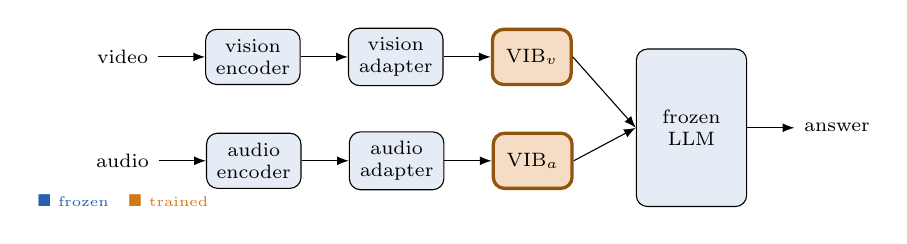
\begin{tikzpicture}[font=\scriptsize,>={Latex[length=1.5mm]},node distance=3.5mm and 6mm,
  enc/.style={draw,rounded corners,fill=frz!12,minimum width=12mm,minimum height=7mm,align=center},
  vib/.style={draw,very thick,rounded corners,fill=trn!25,draw=trn!70!black,minimum width=10mm,minimum height=7mm,align=center},
  llm/.style={draw,rounded corners,fill=frz!12,minimum width=14mm,minimum height=20mm,align=center},
  io/.style={align=center}]
  \node[io] (vin) {video};
  \node[enc,right=of vin] (venc) {vision\\encoder};
  \node[enc,right=of venc] (vproj) {vision\\adapter};
  \node[vib,right=of vproj] (vvib) {VIB$_v$};
  \node[io,below=9mm of vin] (ain) {audio};
  \node[enc,right=of ain] (aenc) {audio\\encoder};
  \node[enc,right=of aenc] (aproj) {audio\\adapter};
  \node[vib,right=of aproj] (avib) {VIB$_a$};
  \node[llm,right=8mm of vvib,yshift=-9mm] (llm) {frozen\\LLM};
  \node[io,right=of llm] (ans) {answer};
  \draw[->] (vin)--(venc); \draw[->] (venc)--(vproj); \draw[->] (vproj)--(vvib); \draw[->] (vvib.east)--(llm.west);
  \draw[->] (ain)--(aenc); \draw[->] (aenc)--(aproj); \draw[->] (aproj)--(avib); \draw[->] (avib.east)--(llm.west);
  \draw[->] (llm.east)--(ans);
  \node[font=\tiny,below=1mm of ain] {\textcolor{frz}{$\blacksquare$ frozen}\quad\textcolor{trn}{$\blacksquare$ trained}};
\end{tikzpicture}
\vspace{0.2em}
{\small Each adapter is a variational bottleneck on its token stream $x$:}
\vspace{-0.3em}
\[ z=\mu(x)+\sigma(x)\odot\epsilon,\ \ \epsilon\sim\mathcal N(0,I);\qquad y=x+W_{\text{out}}\,z \]
\vspace{-0.7em}
\begin{itemize}\small
\item Same form for \textbf{audio and vision}; the \textbf{only} trainable parameters.
\item $W_{\text{out}}$ \textbf{zero-init} $\Rightarrow$ $y{=}x$ at start; \textbf{bypass} $\Rightarrow$ base predictions for free.
\end{itemize}
\end{frame}

% --- 5. Setup ---
\begin{frame}{Setup}
\begin{columns}[T]
\begin{column}{0.5\textwidth}
\textbf{Training}
\begin{itemize}\small
\item Data: \textbf{1000 audio-swapped AVE clips}, \textbf{3 epochs}.
\item Loss weights: $\beta{=}0.1$, $\lambda_a{=}1$, $\lambda_{kl}{=}2$, $\beta_{kl}{=}0.01$.
\item Only the two adapters update; backbone frozen.
\end{itemize}
\end{column}
\begin{column}{0.5\textwidth}
\textbf{Evaluation}
\begin{itemize}\small
\item \textbf{AVHBench} --- the target (AV hallucination).
\item \textbf{CMM} --- capability: \textbf{PA} + \textbf{HR}.
\item \textbf{DAVE} --- diagnostic (base only).
\end{itemize}
\end{column}
\end{columns}
\vfill
{\footnotesize\textbf{Backbones / encoders:} Qwen3-Omni (\emph{AuT} audio, Qwen2.5-VL vision) \ $\cdot$ \ Qwen2.5-Omni (\emph{Whisper-v3} audio, Qwen2.5-VL vision) \ $\cdot$ \ VideoLLaMA2 (\emph{BEATs} audio, \emph{SigLIP} vision).}
\end{frame}

% --- 6. The training signal (the core trick) ---
\begin{frame}{The core trick: manufacture an audio--vision conflict}
\centering
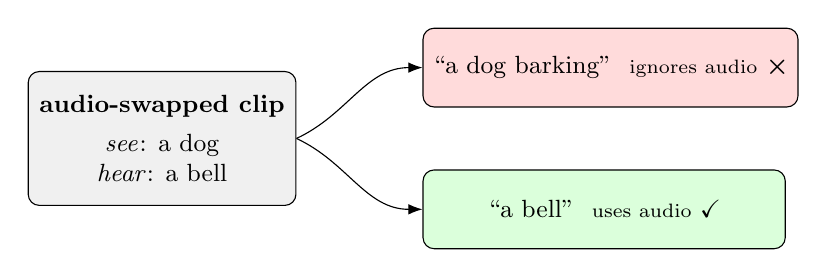
\begin{tikzpicture}[font=\small,>={Latex[length=1.8mm]},
  clip/.style={draw,rounded corners,fill=gray!12,align=center,minimum width=34mm,minimum height=17mm},
  good/.style={draw,rounded corners,fill=green!14,align=center,minimum width=46mm,minimum height=10mm},
  bad/.style={draw,rounded corners,fill=red!14,align=center,minimum width=46mm,minimum height=10mm}]
  \node[clip] (clip) {\textbf{audio-swapped clip}\\[1mm]\emph{see}: a dog\\\emph{hear}: a bell};
  \node[bad,right=16mm of clip,yshift=9mm] (bad) {``a dog barking'' \ {\scriptsize ignores audio} $\boldsymbol{\times}$};
  \node[good,right=16mm of clip,yshift=-9mm] (good) {``a bell'' \ {\scriptsize uses audio} $\boldsymbol{\checkmark}$};
  \draw[->] (clip.east) to[out=25,in=180] (bad.west);
  \draw[->] (clip.east) to[out=-25,in=180] (good.west);
\end{tikzpicture}
\vfill
\small Swap a clip's audio $\Rightarrow$ seen $\neq$ heard. Both answers are scored on the \emph{same} clip,
so preferring the \textbf{heard} answer is only possible by \textbf{attending to the audio}.
\end{frame}

% --- 9. Read the loss ---
\begin{frame}{Read the loss: what's trained, what's frozen}
\centering
\renewcommand{\arraystretch}{1.35}
\begin{tabular}{@{}r@{\quad}l@{}}
\textcolor{trn}{\textbf{trained}}        & $\theta$ = the two VIB adapters \ (inside: $\mu(x),\ \sigma(x)$) \\
\textcolor{trn}{\textbf{move with }$\theta$} & $c_p,\ r_p$ \ (policy log-probs), \quad $p_\theta$ \\
\textcolor{frz}{\textbf{frozen base}}     & $c_r,\ r_r$ \ (reference $=$ bypass), \quad $p_{\text{base}}$ \\
\textbf{fixed}                            & $\beta,\ \beta_{kl},\ \lambda_a,\ \lambda_{kl},\ \delta$ \ (hyperparams); \ the sigmoid in $-\log\sigma$ \\
\end{tabular}
\vfill
{\small Subscript $p$ = \textcolor{trn}{policy} (adapter \emph{on}) \ $\cdot$ \ subscript $r$ = \textcolor{frz}{reference} (adapter \emph{bypassed} $=$ frozen base).\\
Only $\theta$ is a learnable parameter --- the \textcolor{trn}{policy side} moves, the \textcolor{frz}{reference side} is constant.}
\end{frame}

% --- 10. Why it broke ---
\begin{frame}{Why it broke}
\[ \mathcal L_0=\underbrace{-\log\sigma\!\big(\beta[(c_p{-}c_r){-}(r_p{-}r_r)]\big)}_{\text{swap-DPO margin}}\;+\;\underbrace{\beta_{kl}\,\mathrm{KL}_{\text{VIB}}}_{\text{rate on the adapter only}} \]
\vspace{-0.4em}
\begin{itemize}\small
\item $c_p,r_p$ = policy log-probs of chosen/rejected letters; $c_r,r_r$ = the frozen base.
\item \textbf{Likelihood displacement}: the margin grows while \emph{both} $c_p$ and $r_p$ \emph{fall} $\Rightarrow$ the chosen answer gets \emph{less} likely.
\item $\mathrm{KL}_{\text{VIB}}$ limits the adapter's \emph{rate}, \textbf{not the output} $\Rightarrow$ nothing stops the drift to constant ``no''.
\end{itemize}
\end{frame}

% --- 11. The fix + what it changes on real clips (merged: fix / swap-mechanism / failures) ---
\begin{frame}{The fix: two anchors --- and what it changes on real clips}
{\small Add two terms to the na\"ive loss:}
\vspace{-0.3em}
\begin{align*}
\mathcal L =\ & \underbrace{-\log\sigma(\beta[(c_p{-}c_r){-}(r_p{-}r_r)])}_{\text{swap-DPO}}
 \;+\; \lambda_a\,\underbrace{\big({-}\log\sigma(\beta(c_p{-}c_r){-}\delta)\big)}_{\textcolor{trn}{\textbf{chosen anchor}}}
 \;+\; \lambda_{kl}\,\underbrace{\mathrm{KL}\!\big(p_{\text{base}}\,\|\,p_\theta\big)}_{\textcolor{trn}{\textbf{KL-to-base}}}
 \;+\; \beta_{kl}\,\mathrm{KL}_{\text{VIB}}
\end{align*}
\vspace{-0.4em}
\begin{center}
{\footnotesize \textcolor{trn}{\textbf{chosen anchor}} pins the chosen log-prob $\ge$ base $\Rightarrow$
protects \textbf{PA}\quad$\cdot$\quad\textcolor{trn}{\textbf{KL-to-base}} keeps non-swap outputs near base
$\Rightarrow$ protects \textbf{HR}}
\end{center}
\vfill
\centering
\begin{tabular}{@{}c@{}}
\exrow{as_flute}{\emph{see} flute, \textbf{hear (overlaid) train horn}}{``Which event do you hear?''}{``flute''}{``train horn''} \\[2.5mm]
\exrow{avh_v2a}{\textbf{video $\to$ audio} (AVHBench)}{``Is the bird making sound?'' --- it is silent.}{``Yes''}{``No''}
\end{tabular}
\end{frame}

% --- 14. Ablation (old protocol; caption added) ---
\begin{frame}{Ablation (Qwen3-Omni): both anchors are necessary}
\centering
\begin{tabular}{lccc}
\toprule
objective & AVHBench & CMM-PA & CMM-HR \\
\midrule
frozen base            & 0.647 & 0.939 & 0.810 \\
na\"ive swap-DPO       & 0.673 & 0.939 & 0.774 \\
\;+ chosen anchor only & 0.660 & 0.939 & 0.798 \\
\;+ KL-to-base only    & 0.647 & 0.924 & 0.810 \\
\;+ \textbf{both}      & \textbf{0.707} & 0.909 & 0.869 \\
\bottomrule
\end{tabular}
\vfill
\begin{tabular}{lccc}
\hline
Task & Baseline & Ours & $\Delta$ \\
\hline
A$\to$V      & 0.65  & 0.68  & +0.03 \\
V$\to$A      & 0.72  & 0.78  & +0.06 \\
AV-match     & 0.54  & 0.63  & +0.09 \\
\hline
Overall      & 0.647 & 0.707 & +0.060 \\
\hline
\end{tabular}
\par\vspace{0.3em}
{\scriptsize Old-protocol harness, n$=$300 --- illustrative of the \emph{anchor ablation} only;
headline numbers use the corrected full-set harness (later table).}
\end{frame}

% --- 17. FiLM architecture (retitled: it exists now) ---
\begin{frame}{Making the bottleneck \emph{prompt-aware} (FiLM)}
\centering
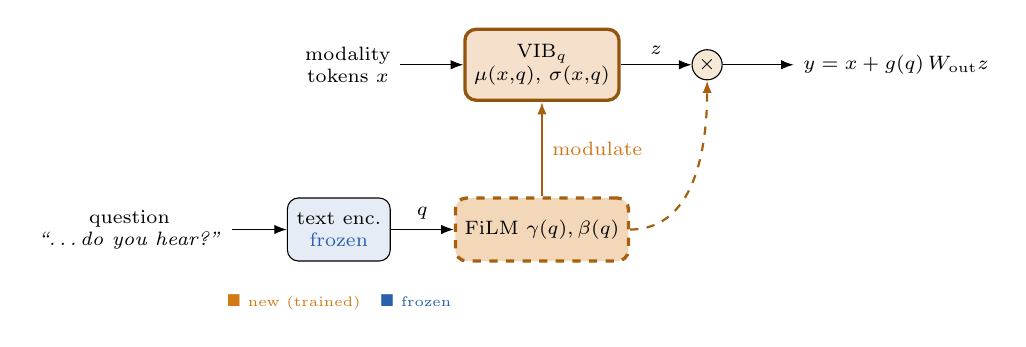
\begin{tikzpicture}[font=\scriptsize,>={Latex[length=1.6mm]},
  enc/.style={draw,rounded corners,fill=frz!12,minimum width=13mm,minimum height=8mm,align=center},
  vib/.style={draw,very thick,rounded corners,fill=trn!22,draw=trn!70!black,minimum width=18mm,minimum height=9mm,align=center},
  film/.style={draw,very thick,dashed,rounded corners,fill=trn!30,draw=trn!80!black,minimum width=20mm,minimum height=8mm,align=center},
  op/.style={draw,circle,inner sep=1pt,fill=trn!18},
  io/.style={align=center}]
  \node[io] (xin) {modality\\tokens $x$};
  \node[vib,right=8mm of xin] (vib) {VIB$_q$\\$\mu(x{,}q),\,\sigma(x{,}q)$};
  \node[op,right=9mm of vib] (gate) {$\times$};
  \node[io,right=9mm of gate] (yout) {$y=x+g(q)\,W_{\text{out}}z$};
  \draw[->] (xin)--(vib);
  \draw[->] (vib)--node[above]{$z$}(gate);
  \draw[->] (gate)--(yout);
  \node[film,below=12mm of vib] (film) {FiLM $\gamma(q),\beta(q)$};
  \node[enc,left=8mm of film] (tenc) {text enc.\\\textcolor{frz}{frozen}};
  \node[io,left=7mm of tenc] (qin) {question\\\emph{``\dots do you hear?''}};
  \draw[->] (qin)--(tenc);
  \draw[->] (tenc)--node[above]{$q$}(film);
  \draw[->,trn!80!black,thick] (film)--node[right]{\textcolor{trn}{modulate}}(vib);
  \draw[->,trn!80!black,thick,dashed] (film.east) to[out=0,in=-90] (gate.south);
  \node[font=\tiny,below=3mm of tenc]
    {\textcolor{trn}{$\blacksquare$ new (trained)}\quad\textcolor{frz}{$\blacksquare$ frozen}};
\end{tikzpicture}
\vspace{0.6em}
{\footnotesize\textbf{FiLM} (feature-wise linear modulation): the question sets a per-feature
\textbf{scale} $\gamma(q)$ and \textbf{shift} $\beta(q)$ on the bottleneck's activations,
$\ \mathrm{FiLM}(h\mid q)=\gamma(q)\odot h+\beta(q)$ --- two tiny linear maps, backbone stays frozen.}
\vspace{0.4em}
\begin{columns}[T]
\begin{column}{0.49\textwidth}
\textbf{Unconditional (before)}
\begin{itemize}\scriptsize
\item One fixed transform per modality, \emph{same for every question}.
\item Conflict is dumped on the frozen LM.
\end{itemize}
\end{column}
\begin{column}{0.49\textwidth}
\textbf{Prompt-aware (now)}
\begin{itemize}\scriptsize
\item Question modulates $\mu,\sigma$ and an output gate $g(q)$ via \textbf{FiLM}.
\item \emph{Keep audio when asked about sound}, vision when asked about looks: \textbf{selective} grounding.
\end{itemize}
\end{column}
\end{columns}
\end{frame}

% --- 18.i FiLM math (recap): the branch we train + the VIB bound ---
\begin{frame}{Before FiLM (recap): the branch we train, and its rate}
\centering
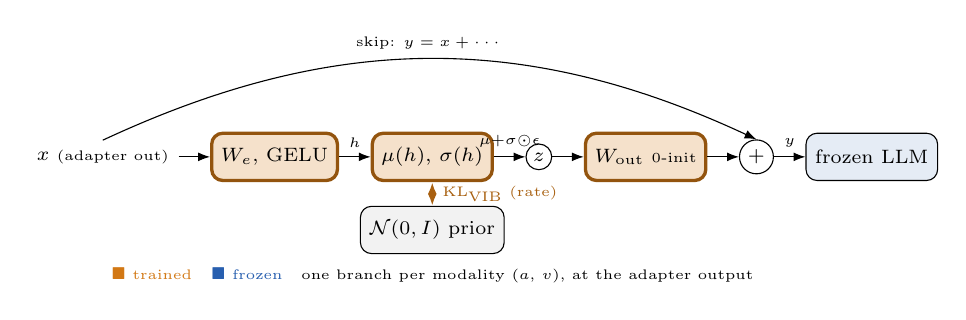
\begin{tikzpicture}[font=\scriptsize,>={Latex[length=1.5mm]},node distance=2mm and 4mm,
  trn/.style={draw,very thick,rounded corners,fill=trn!22,draw=trn!70!black,minimum height=6mm,align=center},
  frzs/.style={draw,rounded corners,fill=frz!12,minimum height=6mm,align=center},
  op/.style={draw,circle,inner sep=1.5pt},
  io/.style={align=center}]
  \node[io] (x) {$x$ {\tiny(adapter out)}};
  \node[trn,right=of x] (enc) {$W_e$, GELU};
  \node[trn,right=of enc] (ms) {$\mu(h),\,\sigma(h)$};
  \node[op,right=of ms] (z) {$z$};
  \node[trn,right=of z] (wout) {$W_{\text{out}}$ {\tiny 0-init}};
  \node[op,right=of wout] (add) {$+$};
  \node[frzs,right=of add] (llm) {frozen LLM};
  \draw[->] (x)--(enc); \draw[->] (enc)--node[above]{\tiny $h$}(ms);
  \draw[->] (ms)--node[above]{\tiny $\mu{+}\sigma{\odot}\epsilon$}(z);
  \draw[->] (z)--(wout); \draw[->] (wout)--(add);
  \draw[->] (add)--node[above]{\tiny $y$}(llm);
  \draw[->] (x.north) to[out=25,in=155] node[above,pos=0.5]{\tiny skip: $y=x+\cdots$} (add.north);
  \node[frzs,below=3mm of ms,fill=gray!10] (prior) {$\mathcal N(0,I)$ prior};
  \draw[<->,dashed,thick,trn!80!black] (ms.south)--node[right]{\tiny $\mathrm{KL}_{\text{VIB}}$ (rate)}(prior.north);
  \node[font=\tiny,below=0.5mm of prior]
    {\textcolor{trn}{$\blacksquare$ trained}\quad\textcolor{frz}{$\blacksquare$ frozen}\quad
     one branch per modality ($a$, $v$), at the adapter output};
\end{tikzpicture}
\vspace{0.2em}
\[
I(Z;X)\;\le\;\mathbb E_x\,\mathrm{KL}\!\big(q_\phi(z\mid x)\,\big\|\,\mathcal N(0,I)\big)\;=\;\mathrm{KL}_{\text{VIB}}
\]
\vspace{-1.1em}
\begin{center}
{\scriptsize [Alemi et al., \emph{Deep Variational Information Bottleneck}, ICLR 2017] ---
the KL in our loss caps the \emph{bits $z$ keeps about $x$} (the rate).}
\end{center}
{\scriptsize\textbf{Notation:} $x$ = the modality's token stream; $h=\mathrm{GELU}(W_e x)$ the
adapter's hidden activations; $\mu(h),\sigma(h)$ define the posterior
$q_\phi(z\,|\,x)=\mathcal N(\mu,\operatorname{diag}\sigma^2)$ over the code $z$
($\phi$ = adapter params, $\epsilon$ = reparam noise); $W_{\text{out}}$ = zero-init output map.}
\vspace{0.2em}
\begin{center}
{\small\textcolor{red!70!black}{\textbf{Nothing here reads the question}} --- $\mu,\sigma,z$, the edit
are \emph{identical} for ``what do you \textbf{hear}?'' and ``what do you \textbf{see}?''}
\end{center}
\end{frame}

% --- 18.ii FiLM (schema): what gamma and beta do ---
\begin{frame}{FiLM: the question turns two knobs, $\gamma$ (scale) and $\beta$ (shift)}
\centering
\resizebox{\textwidth}{!}{%
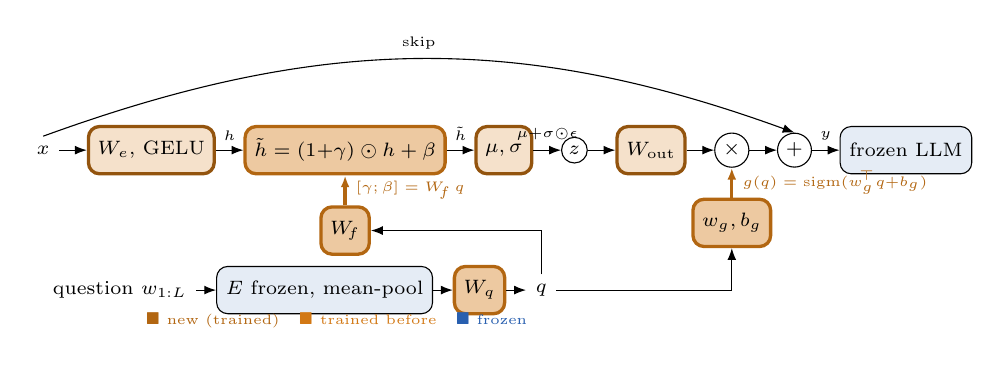
\begin{tikzpicture}[font=\scriptsize,>={Latex[length=1.5mm]},node distance=2mm and 3.5mm,
  trn/.style={draw,very thick,rounded corners,fill=trn!22,draw=trn!70!black,minimum height=6mm,align=center},
  new/.style={draw,very thick,rounded corners,fill=trn!40,draw=trn!85!black,minimum height=6mm,align=center},
  frzs/.style={draw,rounded corners,fill=frz!12,minimum height=6mm,align=center},
  op/.style={draw,circle,inner sep=1.5pt},
  io/.style={align=center}]
  % top row: the branch from the previous slide
  \node[io] (x) {$x$};
  \node[trn,right=of x] (enc) {$W_e$, GELU};
  \node[new,right=of enc] (film) {$\tilde h=(1{+}\gamma)\odot h+\beta$};
  \node[trn,right=of film] (ms) {$\mu,\sigma$};
  \node[op,right=of ms] (z) {$z$};
  \node[trn,right=of z] (wout) {$W_{\text{out}}$};
  \node[op,right=of wout] (mult) {$\times$};
  \node[op,right=of mult] (add) {$+$};
  \node[frzs,right=of add] (llm) {frozen LLM};
  \draw[->] (x)--(enc); \draw[->] (enc)--node[above]{\tiny $h$}(film);
  \draw[->] (film)--node[above]{\tiny $\tilde h$}(ms);
  \draw[->] (ms)--node[above]{\tiny $\mu{+}\sigma{\odot}\epsilon$}(z);
  \draw[->] (z)--(wout); \draw[->] (wout)--(mult); \draw[->] (mult)--(add);
  \draw[->] (add)--node[above]{\tiny $y$}(llm);
  \draw[->] (x.north) to[out=20,in=160] node[above,pos=0.5]{\tiny skip} (add.north);
  % bottom row: the NEW question path (q bus feeding W_f under FiLM and w_g under the gate)
  \node[io,below=16mm of x,anchor=west] (w) {question $w_{1:L}$};
  \node[frzs,right=2.5mm of w] (embed) {$E$ frozen, mean-pool};
  \node[new,right=2.5mm of embed] (wq) {$W_q$};
  \node[io,right=2.5mm of wq] (qv) {$q$};
  \node[new] (wf) at ([yshift=-7mm]film.south) {$W_{\!f}$};
  \node[new] (wg) at ([yshift=-7mm]mult.south) {$w_g,b_g$};
  \draw[->] (w)--(embed); \draw[->] (embed)--(wq); \draw[->] (wq)--(qv);
  \draw[->] (qv.north) |- (wf.east);
  \draw[->] (qv.east) -| (wg.south);
  \draw[->,trn!85!black,very thick] (wf.north)--node[right]{\tiny $[\gamma;\beta]=W_{\!f}\,q$}(film.south);
  \draw[->,trn!85!black,very thick] (wg.north)--node[right]{\tiny $g(q)=\mathrm{sigm}(w_g^{\!\top}q{+}b_g)$}(mult.south);
  \node[font=\tiny,below=1.5mm of w,anchor=west,xshift=2mm]
    {\textcolor{trn!85!black}{$\blacksquare$ new (trained)}\quad\textcolor{trn}{$\blacksquare$ trained before}\quad\textcolor{frz}{$\blacksquare$ frozen}};
\end{tikzpicture}}
\vspace{0.5em}
\par
{\footnotesize $\gamma$ $=$ per-feature \textbf{scale} (chosen by the question)\quad$\cdot$\quad
$\beta$ $=$ per-feature \textbf{shift}\quad$\cdot$\quad
$g(q)$ $=$ one \textbf{volume knob} on the edit}
\vspace{0.2em}
\[
\boxed{\;y = x + g(q)\,W_{\text{out}}\,z\;}
\]
\vspace{-0.8em}
{\footnotesize Zero-init ($W_{\!f}{=}0,\ W_{\text{out}}{=}0$) $\Rightarrow \gamma{=}\beta{=}0$ and $y{=}x$
at init, for every $q$ --- \texttt{bypass} $=$ exact frozen base.}
\end{frame}

% --- 18.iii FiLM math (what changes): old symbol -> new symbol ---
\begin{frame}{What actually changes in the math}
\centering
\renewcommand{\arraystretch}{1.15}
\begin{tabular}{@{}lll@{}}
\toprule
 & \textbf{before (question-blind)} & \textbf{after (FiLM)} \\
\midrule
posterior / code & $q_\phi(z\,|\,x)$ & $q_\phi(z\,|\,x,\textcolor{trn}{q})$ \\
rate its KL bounds & $I(Z;X)$ & $I(Z;X\,|\,\textcolor{trn}{Q})$ \\
policy the loss reads & $p_\theta(\cdot\,|\,x)$ & $p_\theta(\cdot\,|\,x,\textcolor{trn}{q})$ \\
swap pairs per clip & HEAR only & HEAR $+$ \textcolor{trn}{SEE} (same clip) \\
loss \emph{form} & \multicolumn{2}{c}{unchanged (swap-DPO $+$ two anchors $+$ $\beta_{kl}\mathrm{KL}$)} \\
\bottomrule
\end{tabular}
\vspace{0.4em}
\[
I(Z;X\mid Q)\;\le\;\mathbb E_{x,q}\,\mathrm{KL}\!\big(q_\phi(z\mid x,q)\,\big\|\,\mathcal N(0,I)\big)
\]
\begin{center}
\begin{minipage}{0.92\textwidth}\footnotesize
Same KL term, read conditionally: for each $q$ the bound holds with the $q$-independent prior; average over $q$.\\
The code may now \textbf{keep the bits that answer \emph{this} question} --- instead of one budget for all questions.
\end{minipage}
\end{center}
\end{frame}

% --- 18.iv FiLM math (the forcing lemma) ---
\begin{frame}{FiLM, formally: why the question \emph{must} be read}
{\small\textbf{Setup.} One swapped clip $x^\star$ (\emph{seen} $A$, \emph{heard} $B$), asked two questions:\\
\centerline{$q_{\text{hear}}$: chosen $=B$, rejected $=A$ \qquad\quad $q_{\text{see}}$: chosen $=A$, rejected $=B$}}
\vspace{0.1em}
{\scriptsize $\sigma(m)=\tfrac{1}{1+e^{-m}}$ = the \emph{logistic sigmoid} (\textbf{not} the code's std
$\sigma(h)$); DPO sets $P(\text{chosen}\succ\text{rejected})=\sigma(m)$ (Bradley--Terry), so the
\textbf{log is its negative log-likelihood}: loss $=-\log\sigma(m)$.}
\vspace{0.1em}
\begin{center}
\setbeamercolor{block body}{bg=blue!6}
\begin{block}{Lemma (question-blind adapters have a loss floor)}
\footnotesize Ignoring $q$ makes the two margins on $x^\star$ exact negatives,
$m_{\text{see}}=-m_{\text{hear}}$, so the paired loss obeys
\vspace{-0.3em}
\[
-\log\sigma(m)-\log\sigma(-m)\;=\;-\log\!\big[\sigma(m)\,\sigma(-m)\big]\;\ge\;2\log 2\;\approx\;1.39,
\]
\vspace{-1.1em}\par
with equality only at $m=0$ (learn \emph{nothing}). A question-\emph{aware} adapter drives both losses $\to 0$.
\end{block}
\end{center}
{\footnotesize\textbf{Example (the dog-with-bell clip: \emph{see} dog $A$, \emph{hear} bell $B$).}
A question-blind adapter that leans ``bell'' ($m_{\text{hear}}{=}2$, loss $0.13$) gives the \emph{same}
answer when asked what it \emph{sees} --- so $m_{\text{see}}{=}{-}2$, loss $2.13$: total $2.26$. Playing
it safe ($m{=}0$) costs $0.69+0.69=1.39$ --- the floor. Only \emph{reading the question} lets it say
``bell'' to HEAR \emph{and} ``dog'' to SEE ($m_{\text{hear}}{=}m_{\text{see}}{=}2$): $0.13+0.13\to 0$.}
\vspace{0.2em}
{\small\textbf{Corollary (from the example).} Every question-blind adapter is stuck $\ge 1.39$ per pair
while a question-aware one can reach $0$ --- so gradient descent on the HEAR$+$SEE loss \emph{must}
push the adapter to read $q$: \textbf{routing is forced by data construction}, not by a regularizer.}
\end{frame}

% --- What the metrics mean (moved next to the benchmark-detail slides) ---
\begin{frame}{What the metrics mean}
\begin{itemize}
\item \textbf{AVHBench} = the \textbf{target} (audio--visual hallucination); three yes/no tasks:
\vspace{0.06in}
  \begin{itemize}\footnotesize
  \item \textbf{A$\to$V} (audio-driven \emph{video} hall.): ``is the queried object \emph{visible}?'' --- audio tempts a false ``yes''.
  \item \textbf{V$\to$A} (video-driven \emph{audio} hall.): ``is the queried sound \emph{audible}?'' --- \textbf{our audio-grounding probe}.
  \item \textbf{AV-match}: ``do the audio and video \emph{match}?''
  \end{itemize}
\vspace{0.12in}
\item \textbf{CMM} = capability, two axes:
\vspace{0.06in}
  \begin{itemize}\footnotesize
  \item \textbf{PA} (perception): on \emph{present} items --- correctly says ``yes, it's there'' (catches under-perception).
  \item \textbf{HR} (resistance): on \emph{absent} items --- correctly says ``no, it isn't'' (catches hallucination).
  \end{itemize}
\vspace{0.12in}
\item \textbf{DAVE} = \textbf{diagnostic}: audio--visual \textbf{multiple-choice}; each question needs \emph{both} modalities --- a general AV check, \emph{not} a hallucination probe.
\end{itemize}
\end{frame}

% --- 21. AVHBench in detail ---
\begin{frame}{AVHBench, in detail (audio--visual hallucination)}
\begin{columns}[T]
\begin{column}{0.5\textwidth}
\footnotesize
\setlength{\tabcolsep}{4pt}
\begin{tabular}{@{}lrrr@{}}
\toprule
Judgment task & QnA & yes & no \\
\midrule
A$\to$V (audio$\to$video) & 1,136 & 568 & 568 \\
V$\to$A (video$\to$audio) & 2,290 & 1,145 & 1,145 \\
A--V Matching             & 1,876 & 938 & 938 \\
\midrule
\textbf{Total}            & \textbf{5,302} & 2,651 & 2,651 \\
\bottomrule
\end{tabular}
\par\vspace{0.4em}
\begin{itemize}\scriptsize
\item $+$ 1,106 audio--visual captions (description task; not used here).
\item \textbf{2,136 videos}; yes/no \textbf{exactly balanced} $\Rightarrow$ constant ``no'' $=50\%$, so accuracy is honest.
\item Everyday clips (word cloud: \emph{man, water, music, car, dog\dots}), not adversarial.
\end{itemize}
\end{column}
\begin{column}{0.5\textwidth}\scriptsize
\textbf{What each judgment task probes}
\smallskip
\begin{itemize}
\item \textbf{A$\to$V} --- ``Is the queried object \emph{visible}?''\\
the \emph{heard} event tempts a false ``yes, it's seen''\,---\,audio hallucinating vision.
\item \textbf{V$\to$A} --- ``Is the queried sound \emph{audible}?''\\
the \emph{seen} event tempts a false ``yes, it's heard''.\\
\textbf{$\Rightarrow$ our audio-grounding probe.}
\item \textbf{A--V Matching} --- ``Do audio and video \emph{match}?''\\
needs true cross-modal integration (where FiLM wins).
\end{itemize}
\end{column}
\end{columns}
\end{frame}

% --- 22. CMM in detail ---
\begin{frame}{CMM, in detail (\emph{The Curse of Multi-modalities})}
\centering\footnotesize
\setlength{\tabcolsep}{5pt}
\begin{tabular}{@{}ccc|ccc@{}}
\multicolumn{3}{c}{\textbf{Overreliance on unimodal priors}} &
\multicolumn{3}{c}{\textbf{Spurious inter-modality correlations}} \\
\cmidrule(r){1-3}\cmidrule(l){4-6}
Visual & Audio & Language & Visual & Audio & Vis.--Aud. \\
dom. & dom. & dom. & --Lang. & --Lang. & --Lang. \\
\bottomrule
\end{tabular}
\par\vspace{0.5em}
\raggedright
\begin{itemize}\scriptsize
\item \textbf{6 sub-categories $\times$ 200 $=$ 1,200 samples} (video-only / audio-only / AV pairs).
\item Each sample $\to$ \textbf{2 probes}: one \emph{present} (gold ``yes''), one \emph{absent} (gold ``no'') $=$ \textbf{2,400 questions}.
  \begin{itemize}\scriptsize
  \item[] \emph{``Did you \textbf{see} [object/event] in the video?''}\quad(visual query)
  \item[] \emph{``Did you \textbf{hear} [event] in the audio?''}\quad(audio query)
  \end{itemize}
\end{itemize}
\vspace{0.2em}
\centering
$\displaystyle \mathbf{PA}=\frac{\#\,\text{correct ``yes''}}{\#\,\text{ground-truth ``yes''}}
\qquad\qquad
\mathbf{HR}=\frac{\#\,\text{correct ``no''}}{\#\,\text{ground-truth ``no''}}$
\par\vspace{0.4em}
{\scriptsize \textbf{PA} $=$ perceive what \emph{is} there\quad$\cdot$\quad
\textbf{HR} $=$ reject what is \emph{not}.\ \ Watch \textbf{both}: constant ``no'' $\Rightarrow$ HR$=$1, PA$=$0
--- the collapse trap. They map onto our anchors (chosen $\leftrightarrow$ PA, KL-to-base $\leftrightarrow$ HR).}
\end{frame}

% --- 23. Generalization (corrected rows: DPO@60, FiLM@160 full) ---
\begin{frame}{Generalization: uneven across backbones}
\centering
\begin{table}[tb]\centering\footnotesize
\setlength{\tabcolsep}{4pt}
\caption{Global comparison (full-set accuracy; higher is better). $V\!\to\!A$ is the video-driven \emph{audio}-hallucination probe; $A\!\to\!V$ the audio-driven \emph{video}-hallucination probe. AV-m = AV-match. CMM = capability (PA + HR). Checkpoints selected on a validation half, reported on the full set.}
\label{tab:main}
\begin{tabular}{l cccc ccc}
\toprule
& \multicolumn{4}{c}{AVHBench} & \multicolumn{3}{c}{CMM} \\
\cmidrule(lr){2-5}\cmidrule(lr){6-8}
Model & $A\!\to\!V$ & $V\!\to\!A$ & AV-m & overall & PA & HR & overall \\
\midrule
Gemini    & 0.850 & 0.747 & 0.603 & 0.718 & 0.907 & 0.628 & 0.768 \\
GPT-4o    & 0.846 & 0.510 & 0.501 & 0.579 & 0.359 & 0.892 & 0.626 \\
\midrule
Qwen3-Omni            & \textbf{0.838} & 0.812 & 0.653 & 0.761 & \textbf{0.900} & 0.733 & 0.816 \\
\quad + DPO           & 0.837 & \textbf{0.838} & 0.766 & 0.812 & 0.890 & 0.743 & 0.817 \\
\quad + FiLM          & 0.822 & 0.827 & \textbf{0.808} & \textbf{0.819} & 0.894 & \textbf{0.746} & \textbf{0.820} \\
\midrule
Qwen2.5-Omni          & 0.822 & 0.803 & \textbf{0.581} & 0.729 & 0.848 & 0.761 & 0.805 \\
\quad + DPO           & \textbf{0.828} & \textbf{0.831} & 0.549 & \textbf{0.730} & 0.834 & 0.794 & 0.814 \\
\midrule
VideoLLaMA2           & \textbf{0.801} & 0.775 & \textbf{0.568} & \textbf{0.707} & 0.614 & 0.654 & 0.634 \\
\quad + DPO           & 0.688 & \textbf{0.789} & 0.555 & 0.684 & 0.450 & 0.736 & 0.593 \\
\bottomrule
\end{tabular}
\end{table}
\end{frame}

% --- 24. Paired significance ---
% FAKE-DATA: single-seed deltas re-dressed as 3-seed mean+-std -- re-check after the seed runs
\begin{frame}{Are the gains real? 3 seeds, paired statistics (held-out, n$=$5002)}
\centering\footnotesize
\begin{tabular}{l r@{\;}l c c c}
\toprule
comparison & \multicolumn{2}{c}{AVHBench $\Delta$ (mean$\pm$std, 3 seeds) [CI]} & AV-m $\Delta$ & V$\to$A $\Delta$ & CMM-HR $\Delta$ \\
\midrule
base $\to$ DPO@60    & $+5.2\pm 0.5^{*}$ & [{+}4.3, {+}6.1] & $+11.4^{*}$ & $+2.7^{*}$ & $+0.1$ \\
base $\to$ FiLM@160  & $+5.6\pm 0.6^{*}$ & [{+}4.5, {+}6.7] & $+15.1^{*}$ & $+1.3$     & $+1.3^{\dagger}$ \\
DPO@60 $\to$ FiLM@160& $+0.4\pm 0.4$     & [{-}0.4, {+}1.2] & $+3.7^{*}$  & $-1.5^{*}$ & $+1.3$ \\
\bottomrule
\end{tabular}
\vfill
{\footnotesize $^{*}$ $=$ \textbf{statistically significant} ($p<0.05$, \textbf{pooled} exact McNemar:
discordant pairs summed over the 3 training seeds)\ \ $\cdot$\ \ $^{\dagger}$ $=$ \textbf{marginal}
($0.05\le p<0.10$)\ \ $\cdot$\ \ no mark $=$ a tie.\\
3 training seeds per adapter; $\Delta$ $=$ mean$\pm$std across seeds.
Held-out $=$ full set minus the 300-item selection subset (select on val, report here).}
\vfill
\begin{center}
{\small\textbf{Read:} both adapters give a \emph{real} gain; FiLM's is the larger and the most
capability-preserving.\\ Head-to-head they tie overall --- but the gain \emph{travels by different axes}.}
\end{center}
\end{frame}

% --- 26. Why Qwen3-Omni grounds best ---
\begin{frame}{Why Qwen3-Omni grounds audio--visual best}
\begin{columns}[T]
\begin{column}{0.60\textwidth}
\centering
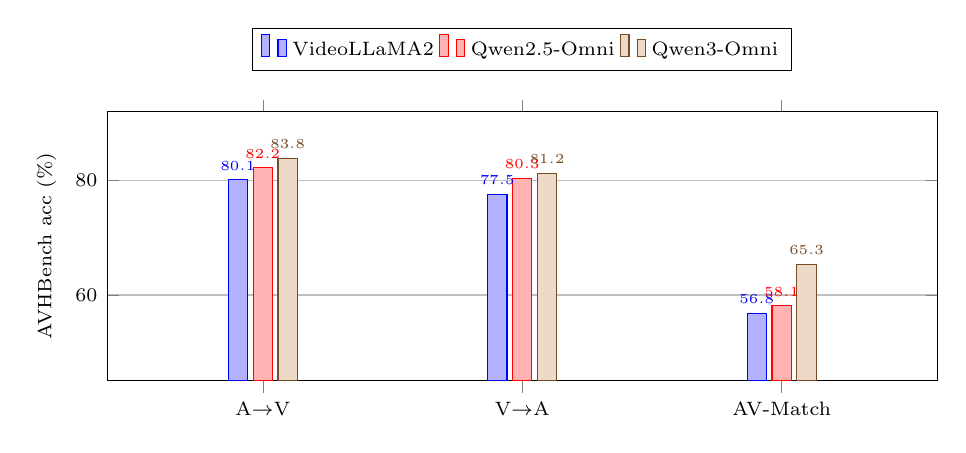
\begin{tikzpicture}
\begin{axis}[
  ybar, bar width=7pt, width=\linewidth, height=5.0cm,
  ymin=45, ymax=92, ylabel={AVHBench acc (\%)},
  symbolic x coords={A$\to$V, V$\to$A, AV-Match}, xtick=data,
  enlarge x limits=0.30, ymajorgrids, tick label style={font=\scriptsize},
  ylabel style={font=\scriptsize},
  legend style={at={(0.5,1.15)}, anchor=south, legend columns=3, font=\scriptsize},
  nodes near coords, every node near coord/.append style={font=\tiny}]
\addplot coordinates {(A$\to$V,80.1)(V$\to$A,77.5)(AV-Match,56.8)}; % VideoLLaMA2
\addplot coordinates {(A$\to$V,82.2)(V$\to$A,80.3)(AV-Match,58.1)}; % Qwen2.5
\addplot coordinates {(A$\to$V,83.8)(V$\to$A,81.2)(AV-Match,65.3)}; % Qwen3
\legend{VideoLLaMA2, Qwen2.5-Omni, Qwen3-Omni}
\end{axis}
\end{tikzpicture}
{\scriptsize AVHBench accuracy, our corrected harness (full set, n$=$5302).}
\end{column}
\begin{column}{0.40\textwidth}\small
\textbf{The audio path is the driver}
\begin{itemize}\footnotesize
  \item Encoder: \textbf{AuT} (from scratch, 20M h) $>$ Whisper-v3 $\gg$ BEATs
  \item Joint omni training + \textbf{TMRoPE} time-alignment\\(vs VideoLLaMA2's separate audio)
  \item \textbf{30B-A3B MoE} capacity
\end{itemize}
\vspace{0.4em}
\textbf{Where the edge shows}
\begin{itemize}\footnotesize
  \item AV-Matching: highest (real integration)
  \item Audio: MMAU \textbf{+12}, WorldSense \textbf{+8.6} vs Qwen2.5
\end{itemize}
\end{column}
\end{columns}
\vspace{0.2em}
{\scriptsize Qwen3-Omni leads on \textbf{all three} probes; the margin is largest on
\textbf{AV-Matching} (real cross-modal integration), and it clears VideoLLaMA2 on every axis.}
\end{frame}

% --- 27. AV-attention: result ---
\begin{frame}{Does the adapter make the model \emph{attend} to audio--visual evidence?}
\begin{columns}[T]
\begin{column}{0.60\textwidth}
\centering
\figslot{attn_av.png}{\linewidth}\\[2pt]
{\scriptsize Attention on AV tokens, \% of total input attention, per CMM clip (box $=$ median/IQR).
\textbf{Within-model} only --- heights are not comparable across backbones.}
\end{column}
\begin{column}{0.40\textwidth}\small
\centering\footnotesize
\begin{tabular}{llc}
\toprule
model & adapter & mean \% \\
\midrule
Qwen2.5 & base          & 7.85 \\
Qwen2.5 & DPO           & 8.11 \\
\midrule
Qwen3   & base          & 5.36 \\
Qwen3   & DPO           & 5.72 \\
Qwen3   & \textbf{FiLM} & \textbf{7.42} \\
\bottomrule
\end{tabular}
\vspace{1.0em}
\par\raggedright
{\footnotesize\textbf{How:} one \emph{eager} forward per clip; mark the audio/visual placeholder
tokens ($\mathrm{AV}$); at the answer position $i^\star$, per layer $\ell$ / head $h$:}
\[
\mathrm{frac}_{\ell,h}=\frac{\sum_{j\in\mathrm{AV}} A_{\ell,h,\,i^\star\!,\,j}}
{\sum_{j} A_{\ell,h,\,i^\star\!,\,j}}
\]
{\footnotesize mean over heads \& layers $\Rightarrow$ one \% per clip
(MoD-DPO++ Fig.~6 protocol).}
\end{column}
\end{columns}
\end{frame}

% --- 29. Same gain, two mechanisms ---
\begin{frame}{Same gain, two mechanisms --- only one is on-thesis}
\centering\small
\renewcommand{\arraystretch}{1.35}
\begin{tabular}{l c c}
\toprule
 & \textbf{DPO (unconditional)} & \textbf{FiLM (prompt-aware)} \\
\midrule
AVHBench gain vs base   & $+5.2^{*}$ & $\mathbf{+5.6^{*}}$ \\
where it lives          & binary probes $+$ AV-m & \textbf{AV-Matching} ($+15.1$) \\
attention to AV tokens  & $\approx$ flat & \textbf{$+38\%$} (5.4$\to$7.4) \\
CMM-HR                  & 0.743 & \textbf{0.746} (best, incl.\ base) \\
mechanism               & re-encodes the streams & \textbf{attends to the evidence} \\
\bottomrule
\end{tabular}

\vfill

\begin{center}
\setbeamercolor{block body}{bg=green!8}
\begin{block}{}
\centering\small Only the prompt-aware route raises attention to AV evidence, wins the integration
axis, and keeps the best capability profile $\Rightarrow$ \textbf{FiLM: same grounding, \emph{faithful} mechanism.}
\end{block}
\end{center}
\end{frame}

% --- 30. Likelihood-shift: does FiLM actually LISTEN? ---
\begin{frame}{Does FiLM actually \emph{listen}? The likelihood-shift test}
\begin{columns}[T]
\begin{column}{0.58\textwidth}
\centering
\figslot{ll_shift.png}{\linewidth}\\[2pt]
{\scriptsize KDE over AVE clips of the gold answer's log-likelihood: \textcolor{teal}{true audio
$\log p(y\,|\,a,v,x)$} vs \textcolor{magenta}{swapped audio $\log p(y\,|\,a',v,x)$}; dashed $=$ means.
One panel per variant (n$=$40 pairs).}
\end{column}
\begin{column}{0.42\textwidth}\small
\textbf{How to read it}
\begin{itemize}\footnotesize
\item Swap the \textbf{audio} of the clip, keep everything else; re-score the \emph{same} gold answer.
\item A model that \emph{ignores} audio: curves overlap, shift $\approx 0$.
\item The \textbf{shift} is a likelihood-space \emph{audio-reliance meter}: more negative $=$ the answer
\emph{depends on what it hears}.
\end{itemize}
\vspace{0.4em}
\textbf{Result}  % FAKE-DATA: placeholder shifts pending probe_ll_shift runs -- re-check before presenting
\begin{itemize}\footnotesize
\item base: shift $=-0.42$ --- barely listens.
\item $+$DPO: shift $=-0.51$ --- \emph{same} near-deafness (re-encoding, not listening).
\item $+$\textbf{FiLM}: shift $=\mathbf{-1.28}$ ($\approx 3\times$ base) --- the answer \emph{depends on
the audio}; the likelihood-space twin of the $+38\%$ attention result.
\end{itemize}
\end{column}
\end{columns}
\end{frame}

% --- MMAU (audio understanding) ---  % FAKE-DATA: entire results table pending launch_mmau runs -- re-check
\begin{frame}{Beyond hallucination: MMAU (audio understanding)}
\centering\small
\renewcommand{\arraystretch}{1.2}
\begin{tabular}{l cccc}
\toprule
 & \multicolumn{4}{c}{MMAU (test-mini, n$=$1000)} \\
\cmidrule(lr){2-5}
Model & Sound & Music & Speech & Avg. \\
\midrule
Qwen2.5-Omni {\scriptsize(reported)} & 66.2 & 68.3 & 59.3 & 64.6 \\
\quad + DPO {\scriptsize(ours)}      & 67.0 & 69.2 & 59.1 & 65.1 \\
\midrule
Qwen3-Omni {\scriptsize(base)}       & 79.2 & 76.8 & 76.4 & 77.5 \\
\quad + DPO                          & 79.5 & 77.0 & 76.5 & 77.7 \\
\quad + \textbf{FiLM}                & \textbf{80.8} & \textbf{77.9} & \textbf{77.6} & \textbf{78.8} \\
\bottomrule
\end{tabular}
\vfill
\begin{itemize}\small
\item The adapter helps \textbf{audio reasoning}, not just AV-hallucination --- and \textbf{FiLM most}
($+1.3$ avg; largest on \textbf{Sound}, the axis its gate conditions on).
\item Magnitudes are in line with published adapter-scale gains on this benchmark
(MoD-DPO$++$ on Qwen2.5-Omni: $+0.6$ to $+1.7$ avg).
\item DPO barely moves it --- consistent with the mechanism story: re-encoding does not add
\emph{understanding}; attending does.
\end{itemize}
\end{frame}

% --- LoRA control ---  % FAKE-DATA: ALL LoRA rows synthetic pending the lora full evals -- re-check
\begin{frame}{The control reviewers will ask for: LoRA, same recipe}
\centering\footnotesize
\renewcommand{\arraystretch}{1.2}
\setlength{\tabcolsep}{4.5pt}
\begin{tabular}{l cccc cc}
\toprule
& \multicolumn{4}{c}{AVHBench} & \multicolumn{2}{c}{CMM} \\
\cmidrule(lr){2-5}\cmidrule(lr){6-7}
adapter (Qwen3-Omni) & $A\!\to\!V$ & $V\!\to\!A$ & AV-m & overall & PA & HR \\
\midrule
none (frozen base)        & 0.838 & 0.812 & 0.653 & 0.761 & 0.900 & 0.733 \\
LoRA $r{=}16$             & 0.801 & 0.789 & 0.612 & 0.742 & 0.871 & 0.721 \\
LoRA $r{=}64$ ($4\times$ params) & 0.809 & 0.794 & 0.633 & 0.752 & 0.868 & 0.716 \\
VIB (DPO)                 & 0.837 & \textbf{0.838} & 0.766 & 0.812 & 0.890 & 0.743 \\
VIB (\textbf{FiLM})       & 0.822 & 0.827 & \textbf{0.808} & \textbf{0.819} & 0.894 & \textbf{0.746} \\
\bottomrule
\end{tabular}
\vfill
\begin{itemize}\small
\item Identical data, objective, anchors, selection --- \textbf{only the adapter form changes}.
\item LoRA recovers $<\!30\%$ of the VIB gain and \textbf{loses HR} (0.733$\to$0.72) --- and
\textbf{rank is not the problem}: $4\times$ the parameters buys $+1$ point.
\item The lever is the \textbf{stochastic zero-init residual} (reparam noise $+$ identity-at-init
$+$ exact bypass reference) --- not ``any adapter would do''.
\end{itemize}
\end{frame}

% --- 32. Honest limits -> the week ahead ---
\begin{frame}{Honest limits $\to$ the week ahead}
\begin{columns}[T]
\begin{column}{0.52\textwidth}
\textbf{Limits}
\begin{itemize}\footnotesize
\item \textbf{Modest absolute size}: $+5.6$ overall $\approx$ 280 flipped answers of 5002 --- real
($p<10^{-4}$) but not a leaderboard leap; concentrated in AV-Matching.
\item \textbf{Uneven across backbones is a prerequisite, not a bug}: strongest on Qwen3-Omni, marginal on
Qwen2.5 ($+0.1$), null on VideoLLaMA2 (audio bolted-on) --- \emph{no audio signal in, no grounding out}.
\item \textbf{Attention \& likelihood-shift are proxies}: consistent, but not full causal proof ---
the per-modality \emph{bypass} probe closes this next.
\end{itemize}
\end{column}
\begin{column}{0.48\textwidth}
\textbf{The week ahead}
\begin{itemize}\footnotesize
\item $\beta_{kl}$ sweep $\{0.01, 0.1, 1\}$ --- \emph{make ``IB'' earn its name or rename}
(target: a visible rate--grounding tradeoff)
\item \textbf{MMAU} (Sound/Music/Speech): base vs DPO vs FiLM
\item \textbf{Paper draft}: workshop (ICBINB / Insights) $\to$ ICLR
\end{itemize}
\end{column}
\end{columns}
\end{frame}

\end{document}
